\documentclass[osajnl,twocolumn,showpacs,superscriptaddress,10pt,floatfix]{revtex4-1} %% use 11pt for Applied Optics
\usepackage{amsmath,amssymb,graphicx,float}
\usepackage{adjustbox}
\usepackage[utf8]{inputenc}
\graphicspath{ {images/} }

\begin{document}

\title{Thyroid Disease Data Set Analysis}

\author{Ulises Jeremias Cornejo Fandos}
\affiliation{Licenciatura en Informatica - 13566/7, Facultad de Informatica, UNLP}

\author{Gaston Gustavo Rios}
\affiliation{Licenciatura en Informatica - 13591/9, Facultad de Informatica, UNLP}


\begin{abstract}
Resumen
\end{abstract}

\maketitle %% required

\section{Introducción}

\subsection{Thyroid Disease Data Set }

El data set cuenta con un conjunto de 6 bases de datos. En general, estos conjuntos son muy similares y presentan muchos atributos, \textit{aproximadamente 29 atributos cada conjunto de datos}, siendo la mayoría booleanos o reales. El dominio del problema es el análisis de enfermedades de tiroides y se utiliza para su estudio un conjunto de datos otorgado por Garavan Institute. Cada conjunto de datos cuenta con aproximadamente 2800 ejemplos y una \textit{gran cantidad de datos faltante}. \\

El conjunto de datos seleccionado permite la clasificación de pacientes entre aquellos que tienen hipotiroidismo y aquellos que no. En su versión presenta un total de 3163 ejemplares de los cuales se conocen 26 atributos. \\

\subsubsection{Información de los atributos}

\begin{itemize}
    \item \textit{age}: Este atributo corresponde a la edad del paciente. En un valor numérico continuo que toma valores de $R$.
    \item \textit{sex}: Este atributo corresponde al sexo del paciente. Toma valores del conjunto $\{M, F\}$ y presenta valores faltante.
    \item \textit{on\_thyroxine}:  \textit{Thyroxine} es la principal hormona generada por la glándula tiroides. Cuando se detecta mucha thyroxine y triyodotironina entonces reduce la producción de hormonas \textit{(TSH)}. Relacionado con goitre, este es una forma de reconocer demasiada thyroxine, la cual es causada por hipertiroidismo. Muy poca es causada por hypotiroidismo. Atributo binominal que toma valores del conjunto $\{f, t\}$.
    \item \textit{query\_on\_thyroxine}: Este atributo indica si fue medido \textit{on\_thyroxine}. Atributo binominal que toma valores del conjunto $\{f, t\}$.
    \item \textit{on\_antithyroid\_medication}: Antithyroid es un medicamento que actúa sobre las hormonas tiroides. Este atributo indica si el paciente toma dicha medicación. Atributo binominal que toma valores del conjunto $\{f, t\}$.
    \item \textit{thyroid\_surgery}: Este atributo indica si el paciente ha tenido una cirugía de tiroides. Atributo binominal que toma valores del conjunto $\{f, t\}$.
    \item \textit{query\_hyphotiroid}: Este atributo indica si le fue consultado al paciente si tenía hipotiroidismo. Atributo binominal que toma valores del conjunto $\{f, t\}$.
    \item \textit{query\_hyperthyroid}: Este atributo indica si le fue consultado al paciente si tenía hipertiroidismo. Atributo binominal que toma valores del conjunto $\{f, t\}$.
    \item \textit{pregnant}: Este atributo indica si el paciente esta transitando un embarazo. Atributo binominal que toma valores del conjunto $\{f, t\}$.
    \item \textit{sick}: Este atributo indica si el paciente estaba enfermo al tomar los datos. Atributo binominal que toma valores del conjunto $\{f, t\}$.
    \item \textit{tumor}: Este atributo indica si el paciente tenía un tumor al tomar los datos. Atributo binominal que toma valores del conjunto $\{f, t\}$.
    \item \textit{lithium}: Atributo binominal que toma valores del conjunto $\{f, t\}$.
    \item \textit{goitre}: Inflamación en el cuello causada por una glándula tiroide agrandada. Atributo binominal que toma valores del conjunto $\{f, t\}$.
    \item \textit{TSH\_measured}: Este atributo indica si se mide el \textit{TSH} del paciente. Atributo binominal que toma valores del conjunto $\{f, t\}$.
    \item \textit{TSH}: Atributo numérico que toma valores de $R$. Representa el nivel de hormonas que tiene en sangre. La TSH le ordena a la glándula tiroides producir y secretar las hormonas tiroideas en la sangre.
    \item \textit{T3\_measured}: Este atributo indica si se mide el \textit{T3} del paciente. Atributo binominal que toma valores del conjunto $\{f, t\}$.
    \item \textit{T3}: Atributo numérico que toma valores de $R$. El mismo mide el nivel de triyodotironina en sangre. Afecta a casi todos los procesos fisiológicos en el cuerpo, incluyendo crecimiento y desarrollo, metabolismo, temperatura corporal y ritmo cardíaco. 
    \item \textit{TT4\_measured}: Este atributo indica si se mide el \textit{TT4} del paciente. Atributo binominal que toma valores del conjunto $\{f, t\}$.
    \item \textit{TT4}: Atributo numérico que toma valores de $R$. El mismo indica el nivel total de thyroxine.
    \item \textit{T4U\_measured}: Este atributo indica si se mide el \textit{T4U} del paciente. Atributo binominal que toma valores del conjunto $\{f, t\}$.
    \item \textit{T4U}: Atributo numérico que toma valores de $R$. T4 uptake. Medida de los sitios de unión de hormonas tiroides desocupados en el TBG. La porción de la hormona tiroidea que queda sin fijar es la encargada de producir la actividad biológica.
    \item \textit{FTI\_measured}: Este atributo indica si se mide el \textit{FTI} del paciente. Atributo binominal que toma valores del conjunto $\{f, t\}$.
    \item \textit{FTI}: Atributo numérico que toma valores de $R$. Free thyroxine index. Estima la cantidad de thyroxine libre circulando utilizando TT4 y T4U.
    \item \textit{TBG\_measured}: Este atributo indica si se mide el \textit{TBG} del paciente. Atributo binominal que toma valores del conjunto $\{f, t\}$.
    \item \textit{TBG}: Atributo numérico que toma valores de $R$. Mide el nivel de glucoproteina. La glucoproteina se une en la circulación sanguínea a las hormonas tiroideas T4 y T3. La porción de la hormona tiroidea que queda sin fijar es la encargada de producir la actividad biológica. 
\end{itemize}

\subsection{Recolección del conjunto de datos}

El conjunto de datos seleccionado se obtiene del repositorio \textit{thyroid disease} del conjunto de data sets para machine learning de \textit{archive.ics.uci.edu}. Como se menciona anteriormente, en el mismo existe una gran cantidad de bases de datos y del mismo se opta por utilizar un conjunto de datos agregado más recientemente. \\

En la descripción del mismo se duda de la integridad de los datos pero se comenta que de igual forma el otorgante es Garavan Institute al igual que el resto de los data sets. A su vez, no dice en ningun momento como es que estos datos son recolectados por lo que al momento de analizar estos datos, solo conocemos las fuentes utilizadas y la entidad otorgante. \\

\section{Pre-procesamiento de datos}
\subsection{Conjunto a analizar}

Como se explica en la sección anterior, existen atributos en los cuales se muestra si fue medido un atributo o no. Dado que los valores de estos coinciden con los datos faltantes se opta por la eliminación de dichos atributos. Al mismo tiempo, la cantidad de datos faltantes para la columna correspondiente al atributo TBG es de $2903$ valores el cual se aproxima a un 92\% del total de valores. Teniendo en cuenta esto, se opta por la eliminación de dicha columna dado que se considera que la misma podría llegar a interferir en el proceso del análisis de los datos, quedando finalmente un total de 19 atributos y 3163 ejemplos. \\

Luego se resuelven los datos faltantes de cada atributo utilizando la media de los mismos para los datos continuos y el valor de mayor frecuencia para los valores nominales. Se mapea el valor correspondiente al atributo sexo para que tome valores del conjunto $\{Male, Female\}$, y aquellos atributos booleanos para que los valores pasen de $f$ a $False$ y de $t$ a $True$. \\

\section{Marco Teórico}

En esta sección se introduce brevemente conceptos básicos necesarios para abordar los contenidos de las siguientes secciones del informe con mayores referencias y capacidad de entendimiento. \\

\subsection{Representaciones Gráficas}

\subsubsection{Diagrama de dispersión}

Un \textbf{diagrama de dispersión} es un tipo de diagrama matemático que utiliza las coordenadas cartesianas para mostrar los valores de dos variables para un conjunto de datos. \\

Se emplea cuando una variable está bajo el control del experimentador. Si existe un parámetro que se incrementa o disminuye de forma sistemática por el experimentador, se le denomina parámetro de control o variable independiente y habitualmente se representa a lo largo del eje horizontal (eje de las abscisas). La variable medida o dependiente usualmente se representa a lo largo del eje vertical (eje de las ordenadas). Si no existe una variable dependiente, cualquier variable se puede representar en cada eje y el diagrama de dispersión mostrará el grado de correlación (no causalidad) entre las dos variables. \\

Un diagrama de dispersión puede sugerir varios tipos de correlaciones entre las variables con un intervalo de confianza determinado. La correlación puede ser positiva (aumento), negativa (descenso), o nula (las variables no están correlacionadas). 

\subsubsection{Diagrama de Caja}

Un \textbf{diagrama de caja}, también conocido como \textit{diagrama de caja y bigotes}, es un gráfico que está basado en cuartiles y mediante el cual se visualiza la distribución de un conjunto de datos. Está compuesto por un rectángulo (la caja) y dos brazos (los bigotes). \\

Es un gráfico que suministra información sobre los valores mínimo y máximo, los cuartiles Q1, Q2 o mediana y Q3, y sobre la existencia de valores atípicos y la simetría de la distribución. Primero es necesario encontrar la mediana para luego encontrar los 2 cuartiles restantes. \\

Un diagrama de cajas proporcionan una visión general de la simetría de la distribución de los datos; si la mediana no está en el centro del rectángulo, la distribución no es simétrica. Son útiles para ver la presencia de valores atípicos también llamados outliers. Pertenece a las herramientas de las estadística descriptiva. Permite ver como es la dispersión de los puntos con la mediana, los percentiles 25 y 75 y los valores máximos y mínimos. Ponen en una sola dimensión los datos de un histograma, facilitando así el análisis de la información al detectar que el 50\% de la población está en los límites de la caja.

\subsubsection{Histograma}

En estadística, un \textbf{histograma} es una representación gráfica de una variable en forma de barras, donde la superficie de cada barra es proporcional a la frecuencia de los valores representados. Sirven para obtener una "primera vista" general, o panorama, de la distribución de la población, o de la muestra, respecto a una característica, cuantitativa y continua (como la longitud o el peso). De esta manera ofrece una visión de grupo permitiendo observar una preferencia, o tendencia, por parte de la muestra o población por ubicarse hacia una determinada región de valores dentro del espectro de valores posibles (sean infinitos o no) que pueda adquirir la característica.

\subsubsection{Diagramas de Barras}

Un \textbf{diagrama de barras} es una forma de representar gráficamente un conjunto de datos o valores, y está conformado por barras rectangulares de longitudes proporcionales a los valores representados. Los gráficos de barras son usados para comparar dos o más valores. Las barras pueden orientarse horizontal o verticalmente.

\subsection{Árbol de decisión}

Modelo descriptivo que, por su forma jerarquica, permite visualizar la organización de los atributos. Se produce a partir de la identificación sucesiva de atributos relevantes. El atributo correspondiente a la clase es cualitativo.

\subsection{Árbol de clasificación}

Es un Arbol de decisión cuyas hojas se refieren al mismo atributo y es discreto.

\subsection{Reglas de clasificación}

Modelo supervisado que apartir de la información busca obtener reglas de la forma: $ A \rightarrow B $. \\

Comparado con el modelo explicado en la subsección anterior, las reglas de clasificación son más compactas que los arboles en donde cada regla puede representar un concepto distinto permitiendo así agregar o quitar reglas dinamicamente.

\subsection{Clustering}

Un algoritmo de agrupamiento (en inglés, clustering) es un procedimiento de agrupación de una serie de vectores de acuerdo con un criterio. Esos criterios son por lo general distancia o similitud. La cercanía se define en términos de una determinada función de distancia, como la euclídea, aunque existen otras más robustas o que permiten extenderla a variables discretas. La medida más utilizada para medir la similitud entre los casos es la matriz de correlación entre los nxn casos. Sin embargo, también existen muchos algoritmos que se basan en la maximización de una propiedad estadística llamada verosimilitud. \\

En el contexto de la Mineria de Datos se lo considera una técnica de aprendizaje no supervisado puesto que busca encontrar relaciones entre variables descriptivas pero no la que guardan con respecto a una variable objetivo. \\

\subsubsection{K-Means}

\textbf{K-means} es un método de agrupamiento, que tiene como objetivo la partición de un conjunto de n observaciones en k grupos en el que cada observación pertenece al grupo cuyo valor medio es más cercano. \\

En la figura \ref{figure:clustering_example} se muestra un ejemplo de aplicación del algoritmo k-means para realizar un agrupamiento de los datos.

\begin{figure}[H]
    \centering
    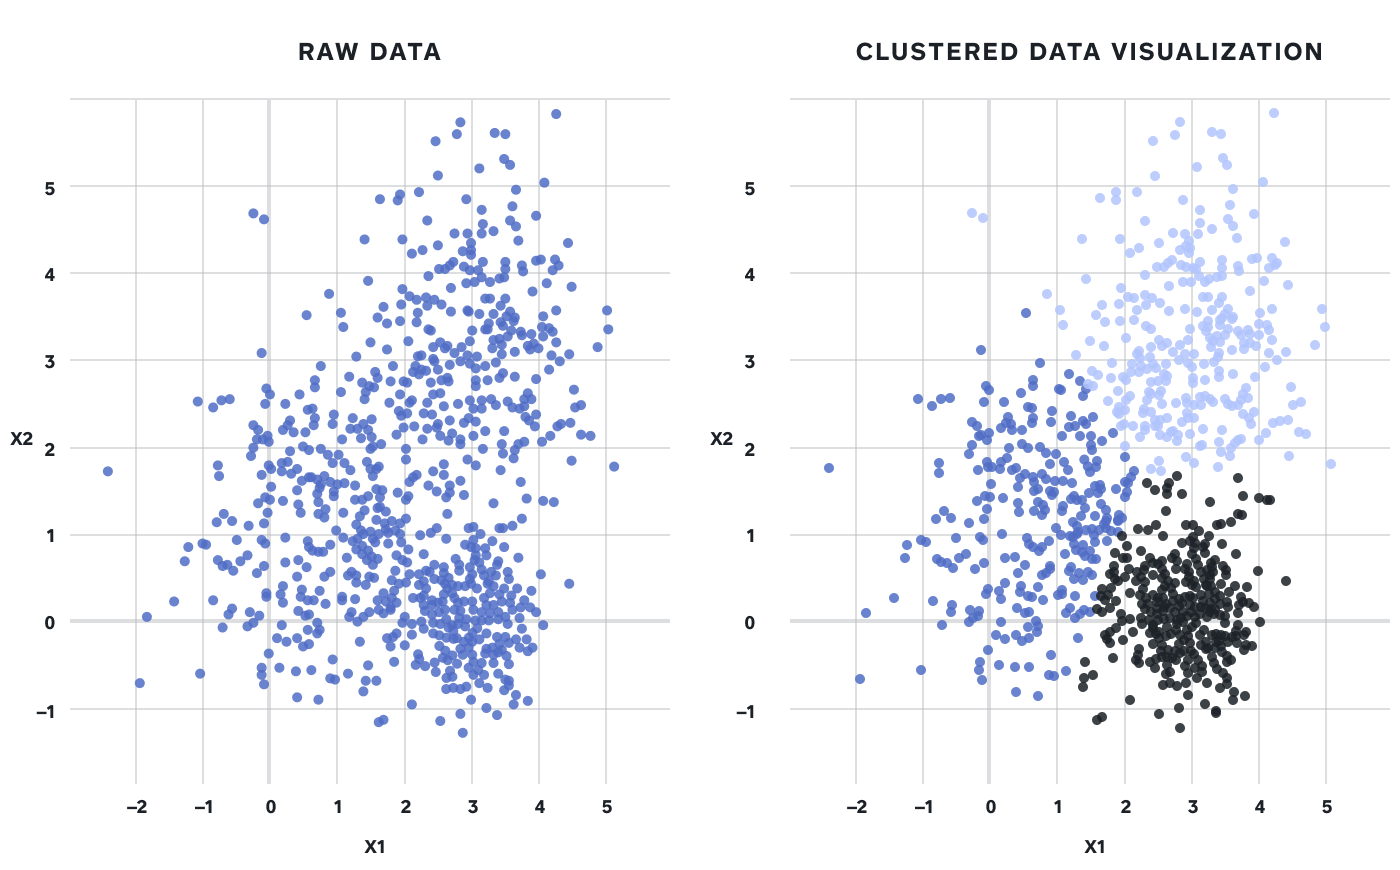
\includegraphics[width=0.4\textwidth]{theory/clustering}
    \caption{Ejemplo de aplicación del algoritmo k-means para realizar un agrupamiento de los datos.}
    \label{figure:clustering_example}
\end{figure}

\subsection{Redes Neuronales}

Las \textbf{redes neuronales} son un modelo computacional basado en un gran conjunto de unidades neuronales simples, \textbf{neuronas artificiales}, de forma aproximadamente análoga al comportamiento observado en los axones de las neuronas en los cerebros biológicos. \\

Cada unidad neuronal está conectada con muchas otras y los enlaces entre ellas pueden incrementar o inhibir el estado de activación de las neuronas adyacentes. Cada unidad neuronal, de forma individual, opera empleando funciones de suma. Puede existir una función limitadora o umbral en cada conexión y en la propia unidad, de tal modo que la señal debe sobrepasar un límite antes de propagarse a otra neurona. \\

Estos sistemas aprenden y se forman a sí mismos, en lugar de ser programados de forma explícita, y sobresalen en áreas donde la detección de soluciones o características es difícil de expresar con la programación convencional.

\subsubsection{Perceptron}

En el campo de las Redes Neuronales, el \textbf{perceptrón}, se refiere a la neurona artificial o unidad básica de inferencia en forma de discriminador lineal, a partir del cual se desarrolla un algoritmo capaz de generar un criterio para seleccionar un sub-grupo a partir de un grupo de componentes más grande. \\

En la figura (\ref{figure:perceptron_example}) se muestra la arquitectura que determina el comportamiento de un perceptron.

\begin{figure}[H]
    \centering
    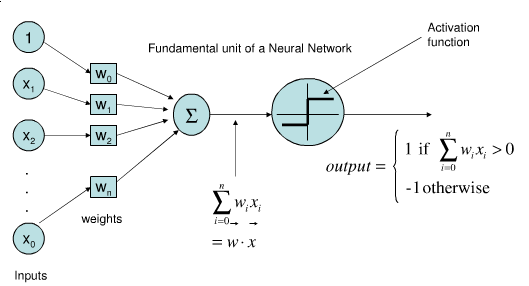
\includegraphics[width=0.4\textwidth]{theory/perceptron}
    \caption{Arquitectura de un perceptron.}
    \label{figure:perceptron_example}
\end{figure}

La limitación de este algoritmo es que si dibujamos en un gráfico estos elementos, se deben poder separar con un hiperplano únicamente los elementos "deseados" discriminándolos (ó \textit{separándolos}) de los \textit{"no deseados"} como se muestra en la figura (\ref{figure:linear_example}).

\begin{figure}[H]
    \centering
    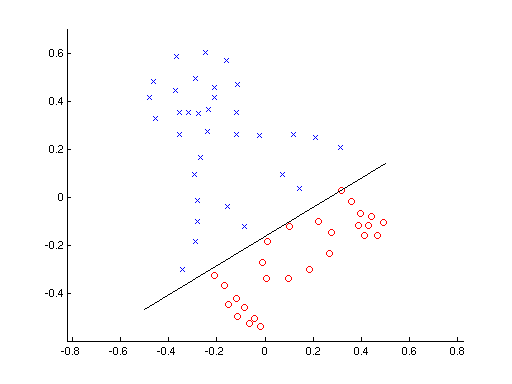
\includegraphics[width=0.4\textwidth]{theory/linear}
    \caption{Ejemplo de función linear discriminante.}
    \label{figure:linear_example}
\end{figure}

El perceptrón puede utilizarse con otros tipos de perceptrones o de neurona artificial, para formar una red neuronal artificial más compleja.

\subsubsection{Multiperceptrón}

El \textbf{perceptrón multicapa}, \textit{multi-perceptrón}, es una red neuronal artificial formada por múltiples capas, de tal manera que tiene capacidad para resolver problemas que no son linealmente separables que, como se explica en la subsección anterior, es la principal limitación del \textit{perceptrón}. El perceptrón multicapa puede estar totalmente o localmente conectado. En el primer caso cada salida de una neurona de la capa \textit{"i"} es entrada de todas las neuronas de la capa \textit{"i+1"}, mientras que en el segundo cada neurona de la capa \textit{"i"} es entrada de una serie de neuronas (región) de la capa \textit{"i+1"}. \\

Se muestra en la figura (\ref{figure:multiperceptron_example}) un ejemplo de la arquitectura de un perceptron multicapa.

\begin{figure}[H]
    \centering
    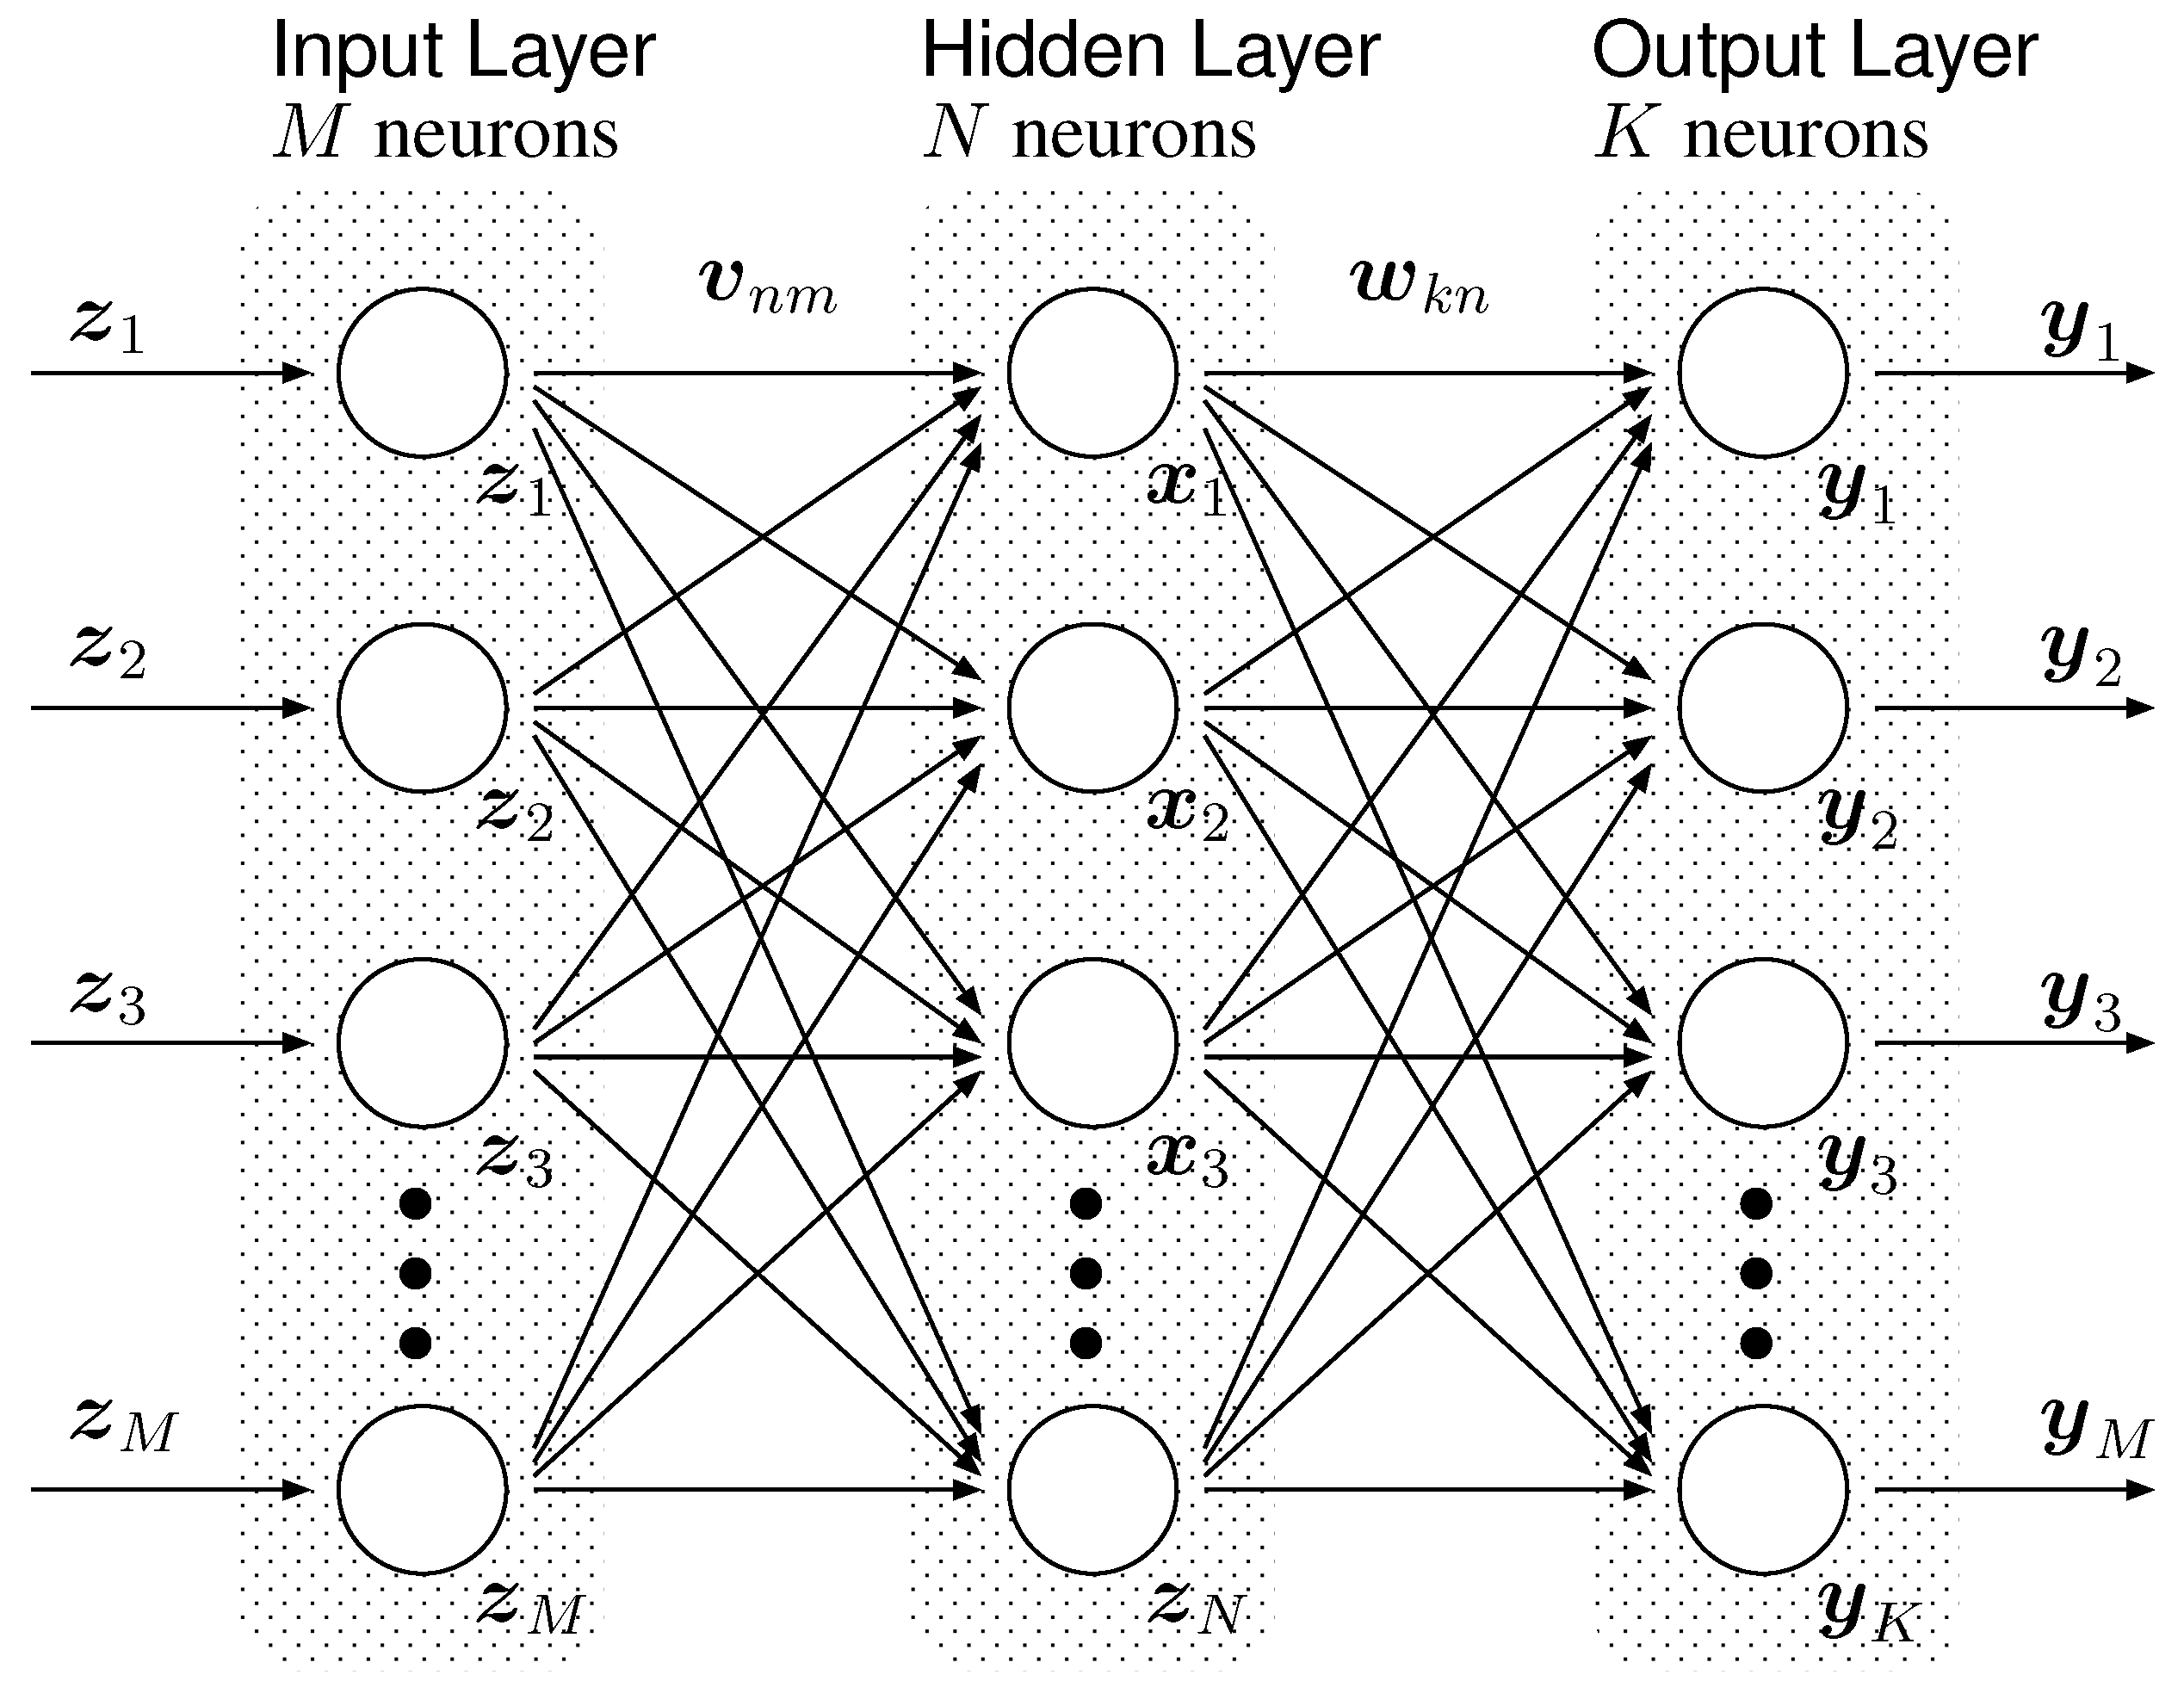
\includegraphics[width=0.4\textwidth]{theory/multiperceptron}
    \caption{Ejemplo básico de un multiperceptron.}
    \label{figure:multiperceptron_example}
\end{figure}

\section{Análisis de datos}

Para el análisis de los datos se evalúan distintas gráficas de los mismos, como graficos de barra de los datos categóricos y gráficas de dispersión e histogramas para aquellos datos de tipo numérico, además de ciertas métricas que permiten conocer la correlación entre cada uno de ellos. De este modo se permite observar relaciones entre los distintos atributos del conjunto de datos así como también la relación entre estos mismos y la etiqueta, o \textit{label}.

\begin{flushright}
\textit{\footnotesize Se dispone de las gráficas correspondientes a los atributos en la sección \ref{apendix:images:attr} del apéndice.}
\end{flushright}

Se puede observar en lo graficos de dispersión que a menor nivel hormonal, ya sea FTI, TT4 o T3, mayor posibilidades existen de tener hipotiroidismo. A su vez, los gráficos de cajas de los atributos numéricos continuos permite observar una gran cantidad de datos fuera de rango extremo pero se cree que esto es normal dado el dominio del problema. \\

Posteriormente, se calcula el índice de correlación lineal entre los atributos, para comenzar así con el análisis de las relaciones entre cada uno de ellos. El cálculo de los mismos se ve reflejado en la siguiente tabla (\ref{table:correlation_matrix}). \\

\begin{table}[h!]
    \centering
    \begin{tabular}{ccccccc}

        Atributos & age & TSH & T3 & TT4 & TU4 & FTI \\
        \hline
        age & 1 & -0.007 & -0.269 & -0.091 & -0.194 & 0.015 \\

        TSH & -0.007 & 1 & -0.172 & -0.310 & 0.069 & -0.244 \\

        T3 & -0.269 & -0.172 & 1 & 0.545 & 0.388 & 0.294 \\

        TT4 & -0.091 & -0.310 & 0.545 & 1 & 0.323 & 0.685 \\

        T4U & -0.194 & 0.069 & 0.388 & 0.323 & 1 & -0.284 \\

        FTI & 0.015 & -0.244 & 0.294 & 0.685 & -0.283 & 1 \\
        \hline
    \end{tabular}
    \caption{Matriz de correlación lineal}
    \label{table:correlation_matrix}
\end{table}

Como se observa en la tabla 1, las tuplas (FTI, TT4) y (T3, TT4) presentan una correlación lineal leve, con un índice de correlación de 0.685 y 0.545 respectivamente. \\

\section{Hipótesis y Objetivos}

Como se menciona anteriormente, en la descripción del data set se cuestiona la integridad de los datos a partir de no poder especificar la procedencia de los mismos y dudar respecto de la entidad otorgante. Es por esto que se tiene como objetivo el poder determinar si estos datos son o no potencialmente útiles para el estudio de las enfermedades de tiroides. Para esto se busca obtener conocimiento que coincida con lo ya sabido sobre el tema y evaluar la posibilidad de generar conocimiento y relaciones nuevas. \\

A partir del análisis de las gráficas, planteadas en la sección anterior, se sabe que cuanto menor sea el nivel de FTI, TT4 y T3, mayor es la posibilidad de tener hipotiroidismo. Sin embargo, no podemos decir lo mismo del TSH dado que no existe una relación obvia de esto. Es por esto que como objetivo se busca confirmar las hipotesis planteadas respecto de las hormonas y determinar la relación entre el TSH y el hipotiroidismo. \\

\section{Método Experimental} \label{section:experimental_method}

En esta sección se detalla todo lo referido al estudio y la creación de los distintos modelos de sistemas inteligentes utilizados para el estudio del conjunto de datos elegido. \\

\subsection{Árbol de decisión}

Para la creación del modelo de Árbol de decisión, se evalúan las distintas posibilidades permitiendo así la construcción de un modelo con un mayor nivel de cobertura sobre el conjunto de datos empleado para entrenamiento y prueba. \\

Se descarta la utilización del criterio de selección ID3 dado que el mismo requiere que los atributos sean nominales y para esto se necesitaria discretizar los valores numéricos. \\

Por lo tanto, como se menciona anteriormente, dado que el conjunto de datos presenta atributos numéricos de tipo continuo, no es completamente viable discretizar los mismos en intervalos si es que existe alguna forma de construir un modelo de Árbol de decisión evitando esto. \\

Se opta finalmente la utilización del algoritmo C4.5 para generar el Árbol de Decisión. Se genera el árbol utilizando el operador W-J48 de rapidminer con la configuración defecto de la mayoría de los flags exceptuando el flag C, \textit{confianza}. Luego de probar distintas configuraciones para el mismo, se observa que dado un conjunto de entrenamiento del 70\% del total de los datos, con un 30\% de los datos destinado al testing del modelo, el porcentaje de acierto del modelo es 99.59\% cuando $C \geq 0.5$, por lo que se configura el flag con $C$ con el valor $0.5$. \\

En la figura (\ref{figure:w_j48}) se puede observar el modelo obtenido utilizando el algoritmo C4.5.

\begin{figure}[H]
    \centering
    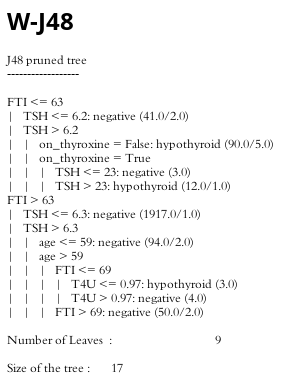
\includegraphics[width=0.35\textwidth]{models/w_j48}
    \caption{Modelo de Árbol generado utilizando el algoritmo C4.5, con una performance de 99.16\%.}
    \label{figure:w_j48}
\end{figure}

En la figura (\ref{figure:w_j48_performance}) de la sección \ref{apendix:models:performance} se puede observar la performance del modelo obtenido aplicando el mismo sobre un conjunto de testing. \\

\subsection{Reglas de Clasificación}

Para definir el algoritmo a utilizar para la creación de reglas se evalúa cada uno de ellos comparando los modelos generados para determinar así cual es más conveniente. Entre los algoritmos evaluados están OneR y PRISM. \\

\subsubsection{OneR}

Se evalúa la construcción del modelo sin normalizar los datos para conocer así el atributo más relevante y punto de inflección en el mismo. El antecedente de la regla generada por este algoritmo se define a partir del atributo $FTI$ como se puede observar en la figura (\ref{figure:w_oneR}) y el principal punto de corte se define cuando FTI toma valores entre $51$ y $62$. \\

\begin{figure}[H]
    \centering
    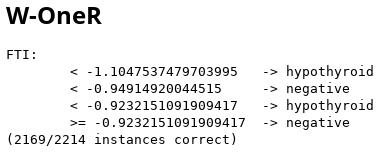
\includegraphics[width=0.35\textwidth]{models/w_oneR}
    \caption{Modelo generado por el algoritmo OneR.}
    \label{figure:w_oneR}
\end{figure}

En la figura (\ref{figure:w_oneR_performance}) de la seccion \ref{apendix:models:performance} se puede observar la performance del modelo obtenido aplicando el mismo sobre un conjunto de testing. \\

\subsubsection{PRISM}

Para la construcción del modelo de reglas utilizando el algoritmo PRISM se discretiza por frecuencia los datos numéricos probando le performance del modelo para distintos intervalos. Finalmente se opta por discretizar en 7 intervalos obteniendo los resultados que se muestran en la figura (\ref{figure:prism_performance}) de la sección \ref{apendix:models:performance}. \\

El algotirmo resulta en un total de 117 reglas de clasificación en las cuales se puede observar que las primeras definidas se ven determinadas por los atributos TSH y FTI, siendo TSH el atributo con mayor frecuencia de aparición en los antecedentes de las primeras reglas.

\section{Clustering}

\subsection{K-Means}

Para la construcción de este modelo se utiliza el algoritmo K-means evaluando las distancias con distancia euclidea. Se normalizan los datos utilizando normalización Z y se evalúa el modelo resultante utilizando el índice de Davies Bouldin notando que se obtiene mejores resultandos cuando el número de clusters $k$ es igual a 2, obteniendo finalmente un índice de Davies Bouldin igual a 0.601. \\

Como resultado se obtienen dos agrupamientos, \textit{cluster\_0} y \textit{cluster\_1}. En los mismos se ve que si el paciente pertenece al cluster\_0 no tiene hypotiroides. Al mismo tiempo, las instancias pertenecientes al cluster\_0 tienen TSH mas bajo, T3 mas alto, y TT4 y FTI bastante más alto que la media. Hay muy pocos que son de cluster\_0 y se pueden ver los datos del agrupamiento en la tabla (\ref{table:k_means}).


\begin{table}[h!]
    \centering
    \begin{tabular}{ccc}
        hypothyroid & cluster & cantidad \\
        \hline
        hypothyroid & cluster\_1 & 151.0 \\
        negative & cluster\_0 & 39.0 \\
        negative  & cluster\_1 & 2973.0 \\
        \hline
    \end{tabular}
    \caption{Resultados del clustering generado con k\_means}
    \label{table:k_means}
\end{table}

Los datos referidos al agrupamiento se pueden ver  en la sección \ref{apendix:models:performance} del apéndice. \\

\section{Redes Neuronales}

Se evalúan distintos modelos de redes neuronales con distintos conjuntos de prueba para evaluar así la performance de los mismos y comparar los modelos resultantes. \\

En ambos casos se normalizan los datos utilizando normalización Z y se aplica dummy coding para transformar los datos nominales. \\

\subsection{Perceptrón}

Dado que el atributo etiqueta del data set es un es un conjunto de valores categóricos de cardinalidad igual a 2, se evalúa la utilización de un perceptrón como posible arquitectura de redes neuronales. \\

\textbf{Pesos y bias}

Como se menciona en el marco teórico, la función discriminante que define al perceptron se define en función de un Intercept y distintos pesos o coeficientes asociados a cada uno de los valores de los atributos del data set. A continuación se enlistan los valores obtenidos luego de entrenar el perceptron. \\

\textit{Intercept} = 1.3490659272630658 \\

En la tabla (\ref{table:perceptron_attr_weight}) se muestran los pesos asociados a cada atributo. \\

\begin{table}[h!]
    \centering
    \resizebox{0.45\textwidth}{!}{
    \begin{tabular}{|ll|ll|}
        \hline
        Atributo & Peso & Atributo & Peso \\
        \hline
        sex = Male & -0.006 & sick = False & -0.019 \\
        sex = Female & 0.006 & sick = True & 0.019 \\
        on\_thyroxine = False & -0.002 & tumor = False & -0.295 \\
        on\_thyroxine = True & 0.002 & tumor = True & 0.295 \\
        query\_on\_thyroxine = False & -0.203 & lithium = False & -1.955 \\
        query\_on\_thyroxine = True & 0.203 & lithium = True & 1.955 \\
        on\_antithyroid\_medication = False & -0.018 & goitre = False & 0.001 \\
        on\_antithyroid\_medication = True & 0.018 & goitre = True & -0.001 \\
        thyroid\_surgery = False & 0.009 & age & -0.016 \\
        thyroid\_surgery = True & -0.009 & TSH & 0.007 \\
        query\_hypothyroid = False & -0.046 & T3 & -0.025 \\
        query\_hypothyroid = True & 0.046 & TT4 & 0.232 \\
        query\_hyperthyroid = False & -0.002 & T4U & -0.102 \\
        query\_hyperthyroid = True & 0.002 & FTI & 0.438 \\
        pregnant = False & -0.052 & & \\
        pregnant = True & 0.052 & & \\
        \hline
    \end{tabular}
    }
    \caption{Tabla de pesos para cada atributo utilizando un perceptrón.}
    \label{table:perceptron_attr_weight}
\end{table}

En las figuras (\ref{figure:perceptron_performance}) y (\ref{figure:perceptron_train_test_performance}) de la seccion \ref{apendix:models:performance} se puede observar la performance del modelo obtenido aplicando el mismo sobre un conjunto de testing. \\

\subsection{Multiperceptron}

Se entrena un multiperceptron utilizando el operador NeuralNet de RapidMiner con 500 ciclos de entrenamiento, 0.03 de tasa de aprendizaje y momentum igual a 0.2, obteniendo una performance mayor a la obtenida con el modelo anterior. \\

En las figuras (\ref{figure:multiperceptron_performance}) y (\ref{figure:multiperceptron_train_test_performance}) de la seccion \ref{apendix:models:performance} se puede observar la performance del modelo de redes neuronales obtenido aplicando el mismo sobre un conjunto de testing. \\

\section{Análisis de Resultados} \label{section:results_analysis}

En esta sección se analizan los resultados obtenidos en el método experimental con el fin de introducir algunos aspectos escenciales para discución de los mismos y conclusiones a tomar. \\

A partir del modelo de arbol de decisión generado es posible observar que el nivel de \textit{FTI} es el atributo que más influye en la discriminación de pacientes permitiendo asó determinar si el mismo tiene hipotiroidismo o no. Si el FTI es bajo y el TSH alto entonces existe grandes posibilidades de que el paciente tenga hipotiroidisme. Esto último permite pensar que, siendo el TSH una hormona que ordena la producción y secreción de hormonas tiroideas, la tiroides realiza una baja producción de hormonas y por lo tanto disminuye el FTI. \\

Este análisis se refuerza con las reglas generadas en las cuales se determina que el atributo FTI es el atributo que más influye en la determinación para poder indicar si, dado un paciente, el mismo poseé o no hipotiroidismo. \\

El agrupamiento obtenido permite obtener información muy importante para el análisis de este problema. En el mismo existe un pequeño grupo de pacientes sin hipotiroidismo con varias características en común. Entre las más importantes encontramos que el nivel de TSH es más bajo, el nivel de T3 y TT4 son mucho más altos, y el nivel de FTI es mucho más alto lo cual indica que están generando una gran cantidad de hormonas a pesar de posser menor nivel de TSH, el cual nos indica el nivel de hormonas que se encarga de estimular su generación. Esto se contradice con los efectos del hipotiroidismo y por lo tanto se puede descartar la posibilidad de que se de este mal. \\

La gran performance generada por el perceptrón indica la posibilidad de separar linealmente a aquellos pacientes con hipotiroidismo de los que no poseen con una gran precisión. Ésta precisión puede ser aumentada aún más utilizando un perceptrón multicapa, llegando a un accuracy igual a $98.52$ sobre un conjunto de datos de testing equivalente al 30\% del total. \\


\section{Discusión y Conclusiones}

A lo largo del método experimental descripto en la sección \ref{section:experimental_method} se obtienen distintos modelos con una gran precisión, lo cual nos permite concluir que es posible estudiar este problema e incluso llegar a predecir de forma eficiente si, dado un paciente, el mismo tiene hipotiroidismo o no. A su vez, se cree que un estudio similar permitiría estudiar otras enfermedades relacionadas con la tiroides así como tambien encontran mayores relaciones entre los atributos de este conjunto de datos concluyendo que el mismo es util para esto a pesar de la cantidad de datos faltantes y las dudas respecto de su integridad. \\

Este data set permite hallar todas las conclusiones mencionadas en la sección \ref{section:results_analysis} observando entre otras cosas que se puede obtener conocimiento ya existente sobre el tema en mucho menor tiempo y a su vez, generar conocimiento nuevo sobre el tema. Se puede decir entonces que a lo largo del análisis se encuentra una relación fuerte entre los atributos tales como el nivel de FTI y TSH, y demás hormonas. De igual forma, se obtienen las carácteristicas que cumple un reducido conjunto de pacientes que no presenta sintomas de hipotiroidismo determinando si un paciente se encuentra sano, o no, con un gran nivel de precisión. \\ 

\begin{thebibliography}{99}

\bibitem{revtex-au} \url{https://authors.aps.org/revtex4/}.
\bibitem{osastyle} \url{http://www.opticsinfobase.org/submit/style/jrnls_style.cfm}.

\end{thebibliography}

\clearpage

\onecolumngrid

\section{Apéndice}

\subsection{Imágenes} \label{apendix:images}

\subsubsection{Gráficos de los atributos} \label{apendix:images:attr}

\twocolumngrid

\begin{figure}[H]
    \centering
    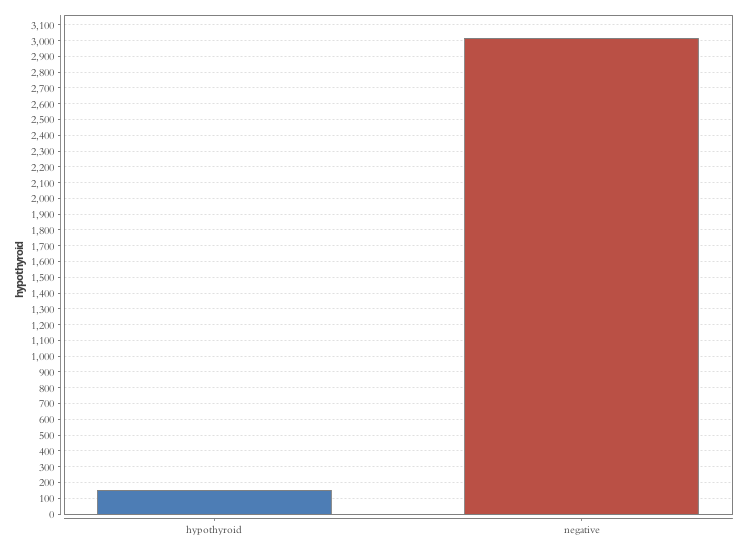
\includegraphics[width=0.45\textwidth]{analysis/bars_hypothyroid}
    \caption{Gráfico de barras del atributo etiqueta.}
    \label{figure:bars_hypothyroid}
\end{figure}

\begin{figure}[H]
    \centering
    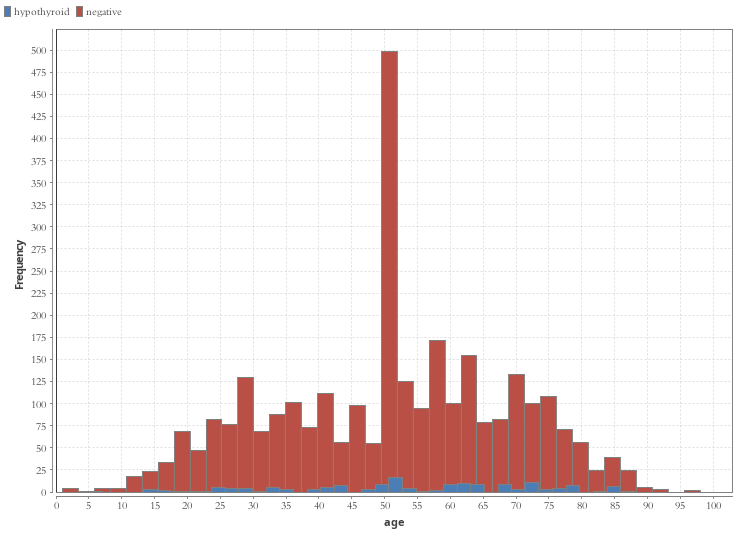
\includegraphics[width=0.45\textwidth]{analysis/histogram_age}
    \caption{Histograma del atributo \textit{age}.}
    \label{figure:histogram_age}
\end{figure}

\begin{figure}[H]
    \centering
    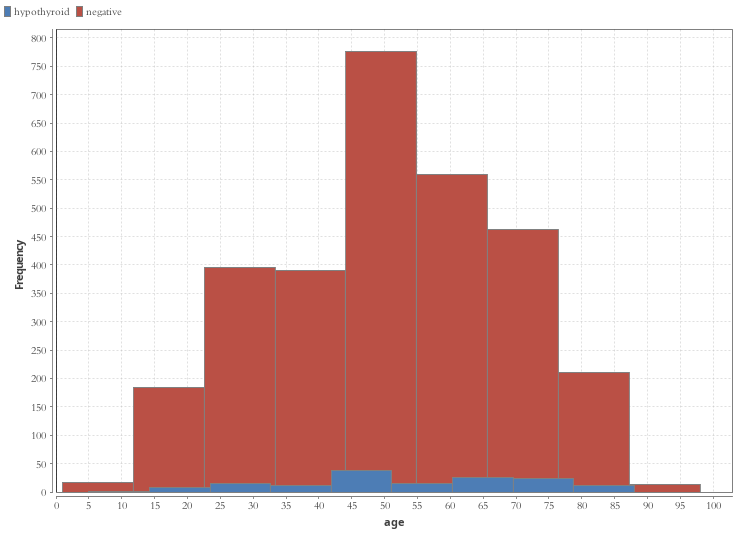
\includegraphics[width=0.45\textwidth]{analysis/histogram_age2}
    \caption{Histograma del atributo \textit{age}.}
    \label{figure:histogram_age2}
\end{figure}

\begin{figure}[H]
    \centering
    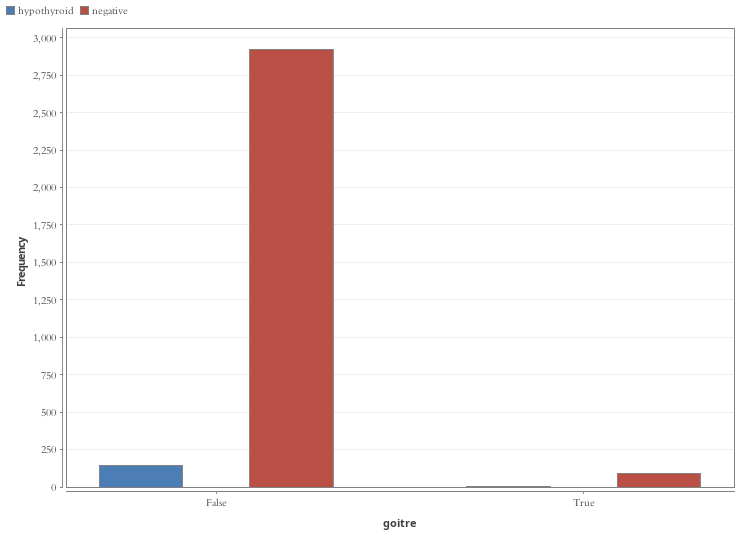
\includegraphics[width=0.45\textwidth]{analysis/histogram_goitre}
    \caption{Histograma del atributo \textit{goitre}.}
    \label{figure:histogram_goitre}
\end{figure}

\begin{figure}[H]
    \centering
    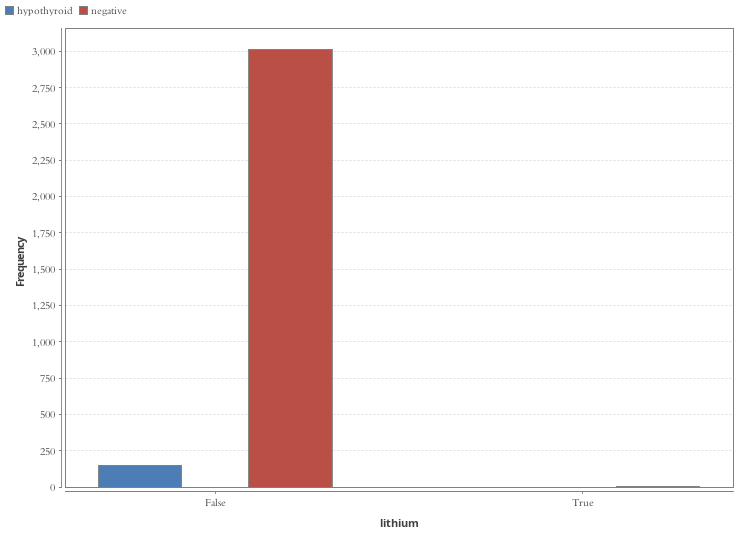
\includegraphics[width=0.45\textwidth]{analysis/histogram_lithium}
    \caption{Histograma del atributo \textit{lithium}.}
    \label{figure:histogram_lithium}
\end{figure}

\begin{figure}[H]
    \centering
    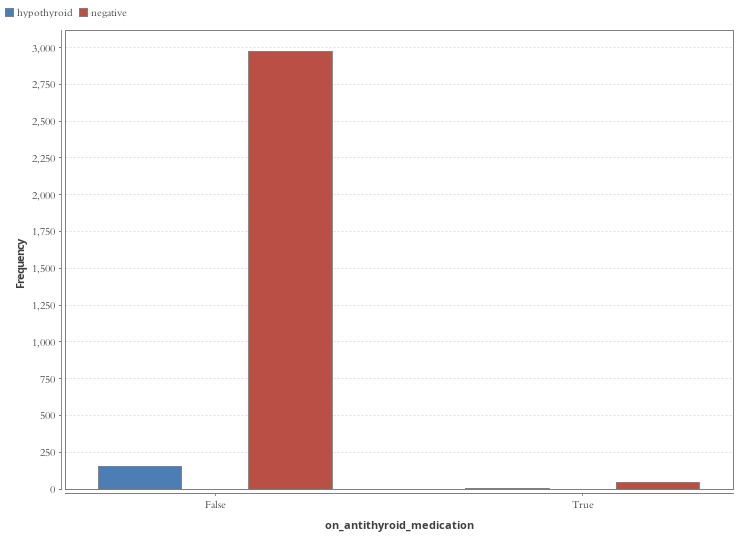
\includegraphics[width=0.45\textwidth]{analysis/histogram_on_antithyroid_medication}
    \caption{Histograma del atributo \textit{on\_antithyroid\_medication}.}
    \label{figure:on_antithyroid_medication}
\end{figure}

\begin{figure}[H]
    \centering
    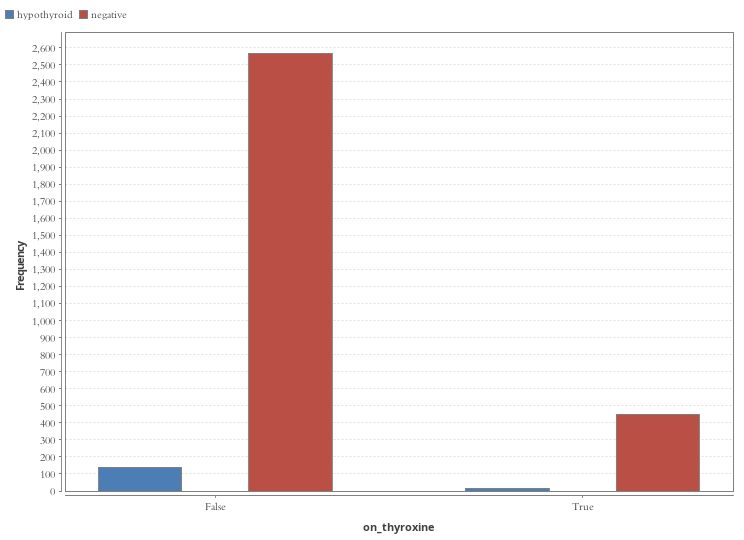
\includegraphics[width=0.45\textwidth]{analysis/histogram_on_thyroxine}
    \caption{Histograma del atributo \textit{on\_thyroxine}.}
    \label{figure:on_thyroxine}
\end{figure}

\begin{figure}[H]
    \centering
    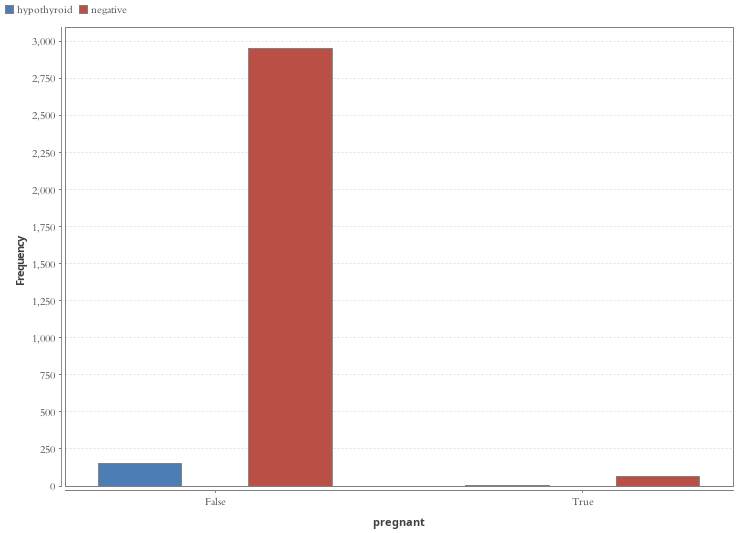
\includegraphics[width=0.45\textwidth]{analysis/histogram_pregnant}
    \caption{Histograma del atributo \textit{pregnant}.}
    \label{figure:pregnant}
\end{figure}

\begin{figure}[H]
    \centering
    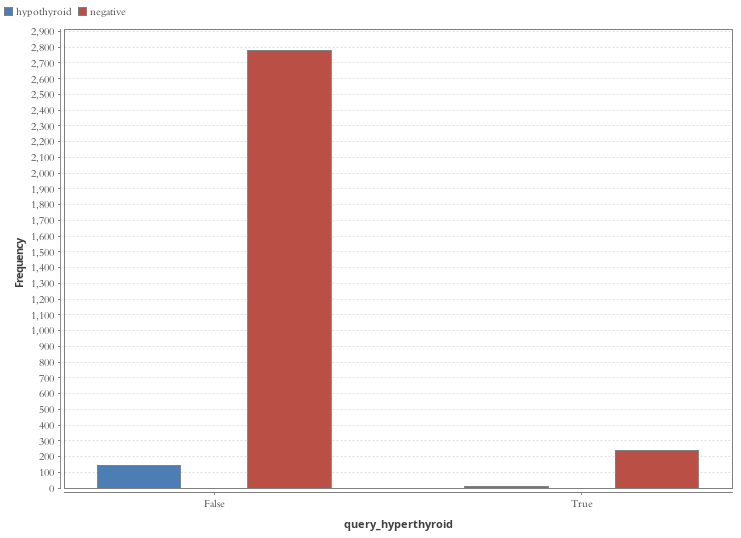
\includegraphics[width=0.45\textwidth]{analysis/histogram_query_hyperthyroid}
    \caption{Histograma del atributo \textit{query\_hyperthyroid}.}
    \label{figure:query_hyperthyroid}
\end{figure}

\begin{figure}[H]
    \centering
    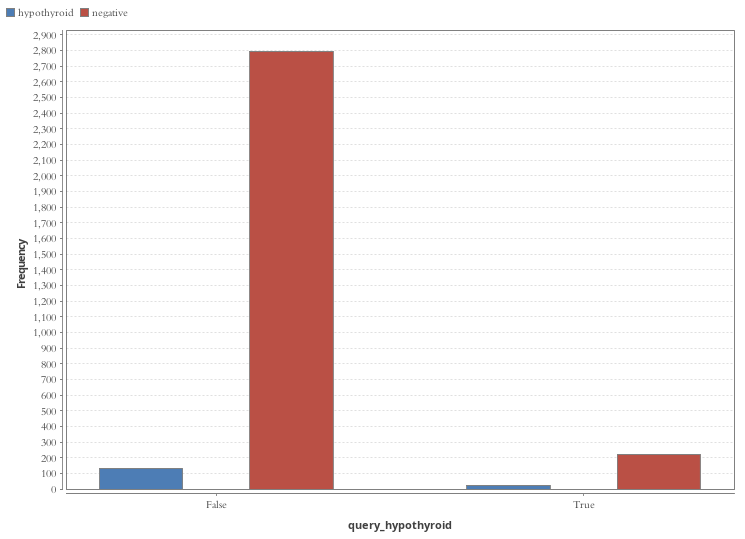
\includegraphics[width=0.45\textwidth]{analysis/histogram_query_hypothyroid}
    \caption{Histograma del atributo \textit{query\_hypothyroid}.}
    \label{figure:query_hypothyroid}
\end{figure}

\begin{figure}[H]
    \centering
    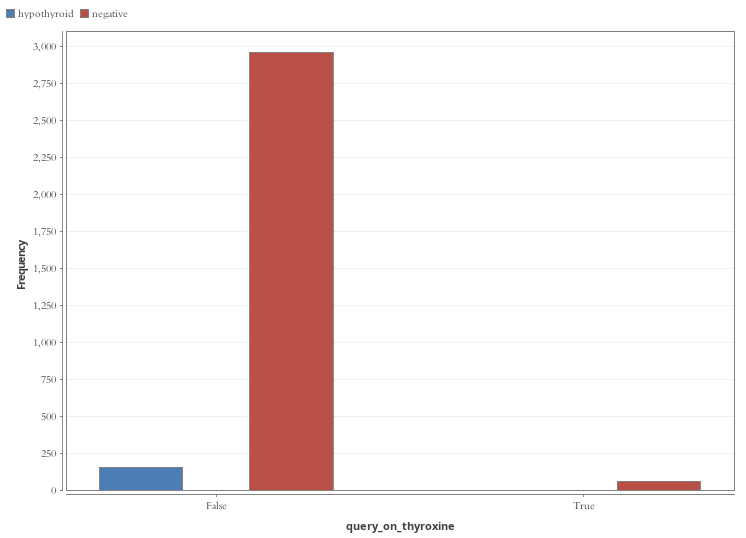
\includegraphics[width=0.45\textwidth]{analysis/histogram_query_on_thyroxine}
    \caption{Histograma del atributo \textit{query\_on\_thyroxine}.}
    \label{figure:query_on_thyroxine}
\end{figure}

\begin{figure}[H]
    \centering
    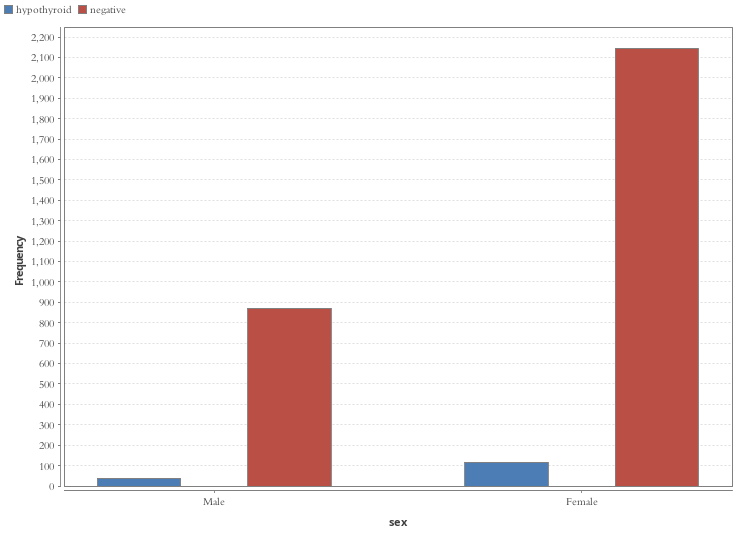
\includegraphics[width=0.45\textwidth]{analysis/histogram_sex}
    \caption{Histograma del atributo \textit{sex}.}
    \label{figure:sex}
\end{figure}

\begin{figure}[H]
    \centering
    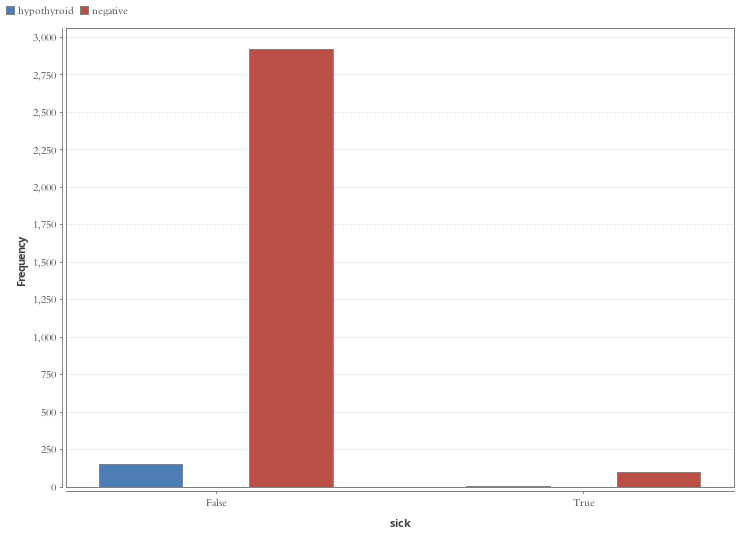
\includegraphics[width=0.45\textwidth]{analysis/histogram_sick}
    \caption{Histograma del atributo \textit{sick}.}
    \label{figure:sick}
\end{figure}

\begin{figure}[H]
    \centering
    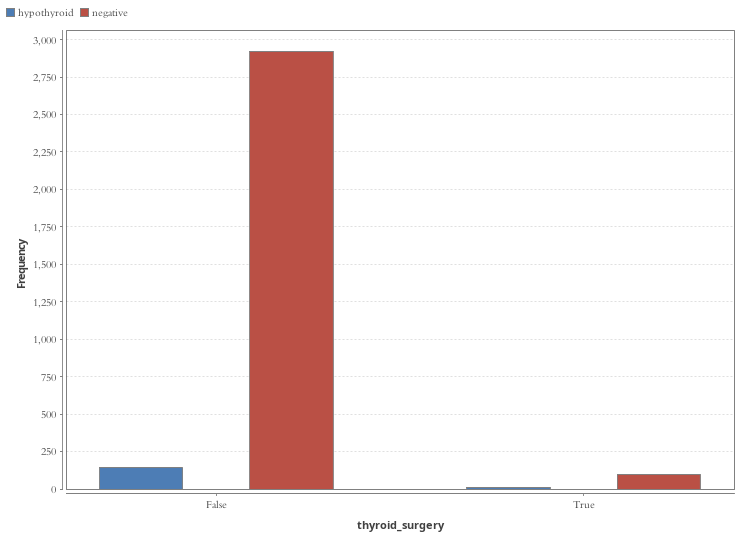
\includegraphics[width=0.45\textwidth]{analysis/histogram_thyroid_surgery}
    \caption{Histograma del atributo \textit{thyroid\_surgery}.}
    \label{figure:thyroid_surgery}
\end{figure}

\begin{figure}[H]
    \centering
    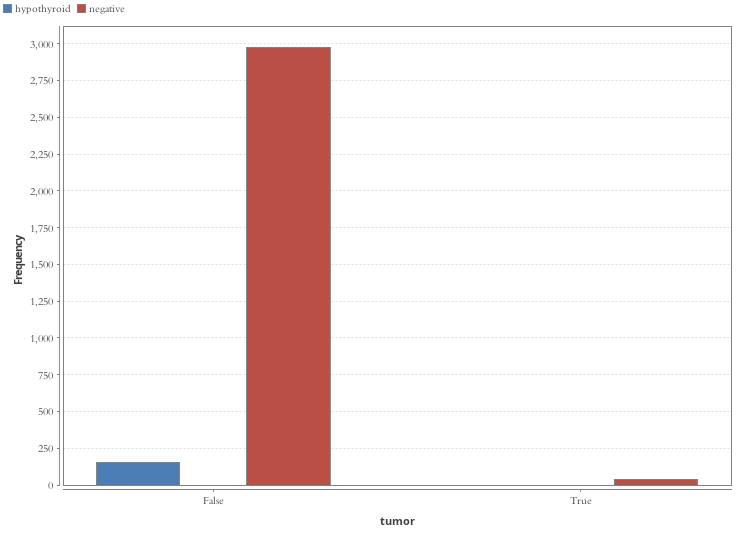
\includegraphics[width=0.45\textwidth]{analysis/histogram_tumor}
    \caption{Histograma del atributo \textit{tumor}.}
    \label{figure:tumor}
\end{figure}

\begin{figure}[H]
    \centering
    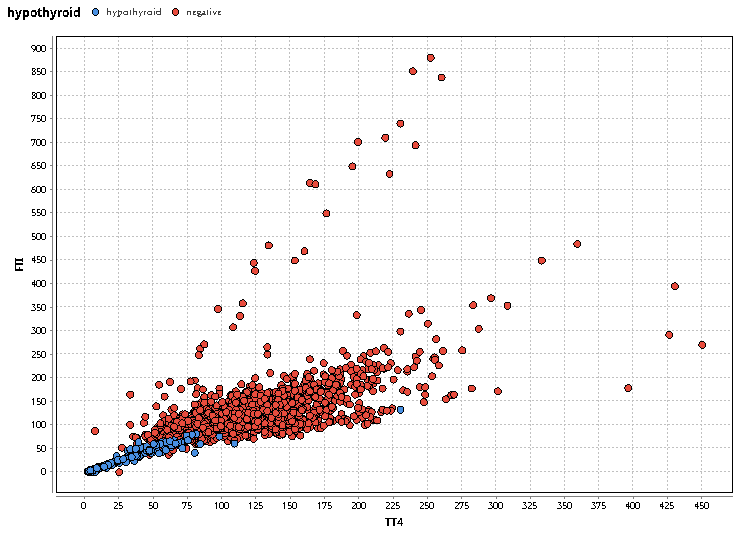
\includegraphics[width=0.45\textwidth]{analysis/scatter_TT4_FTI}
    \caption{Diagrama de dispersión de los atributos \textit{TT4, FTI}.}
    \label{figure:scatter_TT4_FTI}
\end{figure}

\begin{figure}[H]
    \centering
    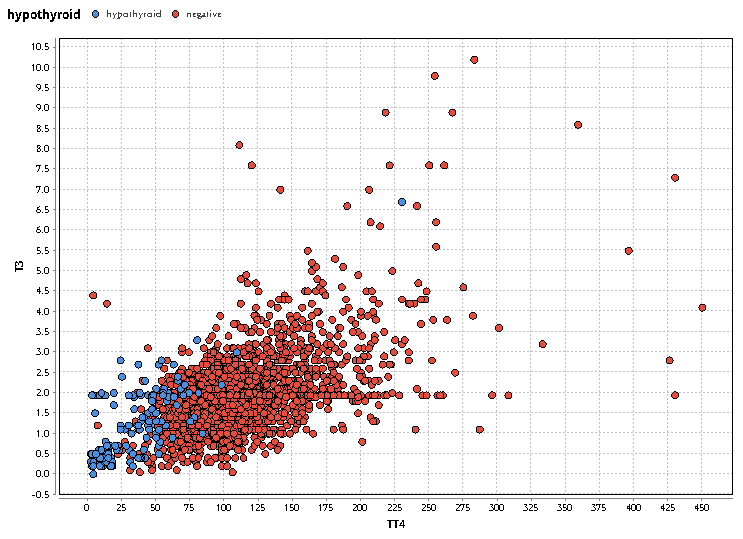
\includegraphics[width=0.45\textwidth]{analysis/scatter_TT4_T3}
    \caption{Diagrama de dispersión de los atributos \textit{TT4, T3}.}
    \label{figure:scatter_TT4_T3}
\end{figure}

\begin{figure}[H]
    \centering
    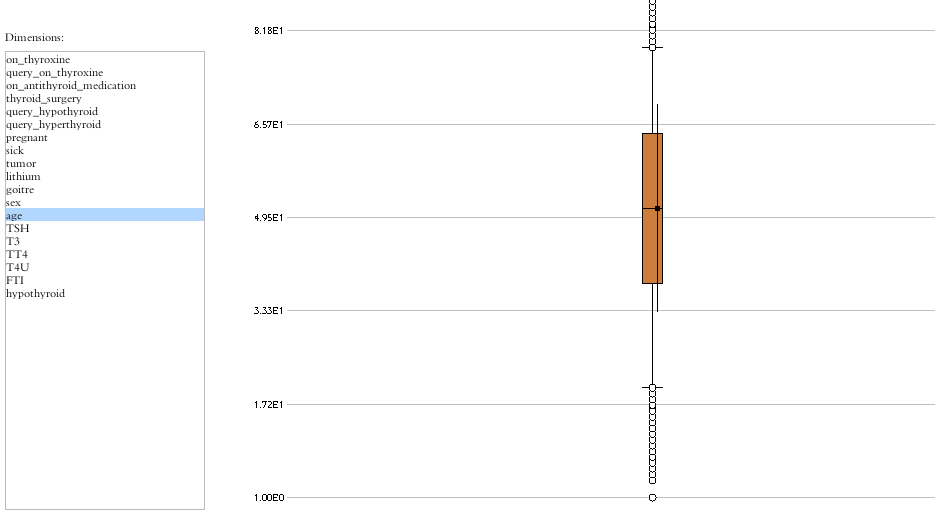
\includegraphics[width=0.45\textwidth]{analysis/box_plot_age}
    \caption{Diagrama de cajas del atributo \textit{age}.}
    \label{figure:box_plot_age}
\end{figure}

\begin{figure}[H]
    \centering
    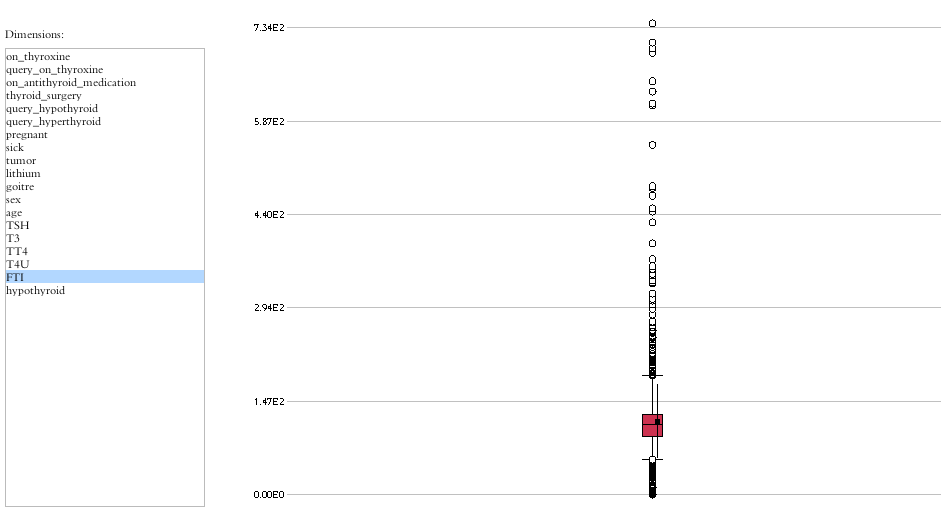
\includegraphics[width=0.45\textwidth]{analysis/box_plot_FTI}
    \caption{Diagrama de cajas del atributo \textit{FTI}.}
    \label{figure:box_plot_FTI}
\end{figure}

\begin{figure}[H]
    \centering
    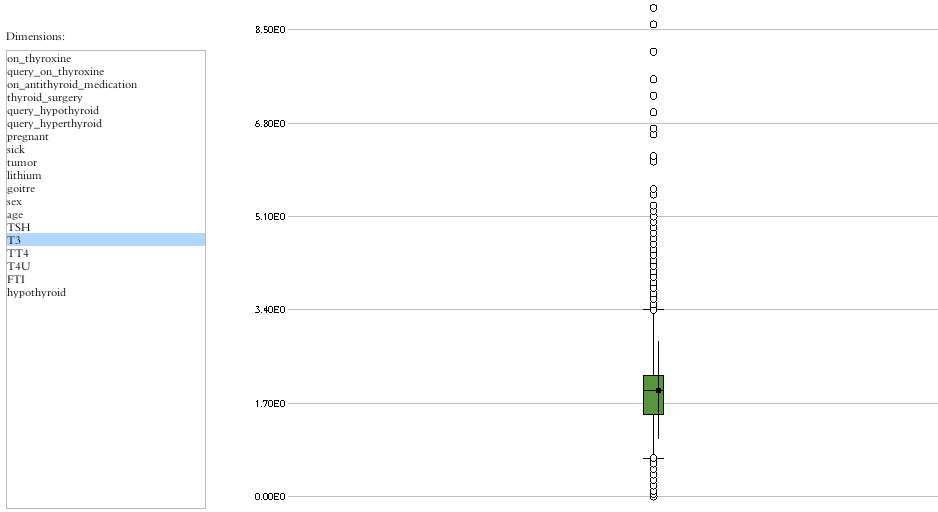
\includegraphics[width=0.45\textwidth]{analysis/box_plot_T3}
    \caption{Diagrama de cajas del atributo \textit{T3}.}
    \label{figure:box_plot_T3}
\end{figure}

\begin{figure}[H]
    \centering
    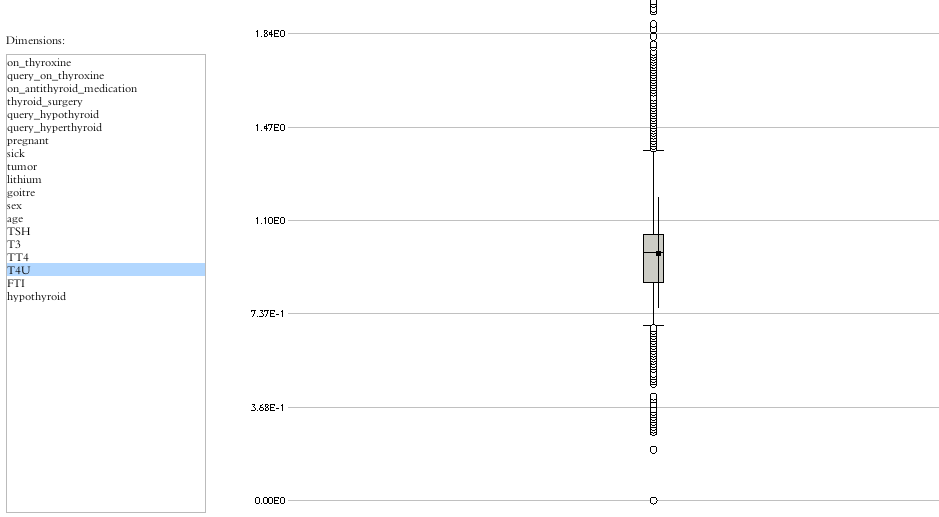
\includegraphics[width=0.45\textwidth]{analysis/box_plot_T4U}
    \caption{Diagrama de cajas del atributo \textit{T4U}.}
    \label{figure:box_plot_T4U}
\end{figure}

\begin{figure}[H]
    \centering
    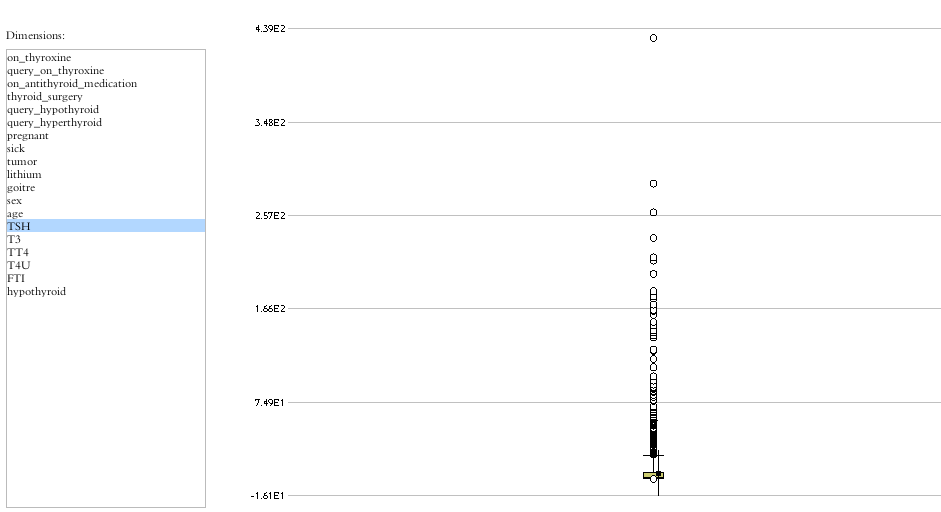
\includegraphics[width=0.45\textwidth]{analysis/box_plot_TSH}
    \caption{Diagrama de cajas del atributo \textit{TSH}.}
    \label{figure:box_plot_TSH}
\end{figure}

\onecolumngrid

\clearpage

\subsection{Modelos y Performance}

\subsubsection{Modelos} \label{apendix:models:models}

\begin{table}[ht]
    \begin{tabular}{|l|l|l|}
        \hline
        Atributo & cluster\_0 & cluster\_1 \\
        \hline

        sex = M & 0.10256410256410256 & 0.2893725992317542 \\
        sex = F & 0.8974358974358975 & 0.7106274007682458 \\
        on\_thyroxine = f & 0.9487179487179487 & 0.8530729833546735 \\
        on\_thyroxine = t & 0.05128205128205128 & 0.1469270166453265 \\
        query\_on\_thyroxine = f & 1.0 & 0.9823943661971831 \\
        query\_on\_thyroxine = t & 0.0 & 0.017605633802816902 \\
        on\_antithyroid\_medication = f & 1.0 & 0.9865556978233034 \\
        on\_antithyroid\_medication = t & 0.0 & 0.013444302176696543 \\
        thyroid\_surgery = f & 1.0 & 0.9667093469910372 \\
        thyroid\_surgery = t & 0.0 & 0.03329065300896287 \\
        query\_hypothyroid = f & 0.9487179487179487 & 0.9234955185659411 \\
        query\_hypothyroid = t & 0.05128205128205128 & 0.0765044814340589 \\
        query\_hyperthyroid = f & 0.6923076923076923 & 0.926056338028169 \\
        query\_hyperthyroid = t & 0.3076923076923077 & 0.07394366197183098 \\
        pregnant = f & 0.9743589743589743 & 0.9801536491677336 \\
        pregnant = t & 0.02564102564102564 & 0.019846350832266324 \\
        sick = f & 1.0 & 0.9683098591549296 \\
        sick = t & 0.0 & 0.03169014084507042 \\
        tumor = f & 1.0 & 0.9871959026888605 \\
        tumor = t & 0.0 & 0.012804097311139564 \\
        lithium = f & 1.0 & 0.9993597951344431 \\
        lithium = t & 0.0 & 6.402048655569782E-4 \\
        goitre = f & 1.0 & 0.9683098591549296 \\
        goitre = t & 0.0 & 0.03169014084507042 \\
        age & 51.51282051282051 & 51.127720870678615 \\
        TSH & 4.964323581180723 & 5.935150321052643 \\
        T3 & 3.487115072933549 & 1.920431471620351 \\
        TT4 & 249.64102564102564 & 107.09236555697822 \\
        T4U & 0.616923076923077 & 0.9827091372498201 \\
        FTI & 472.56410256410254 & 110.93890826408756 \\
        \hline
    \end{tabular}
    \caption{Agrupamiento generado por el algoritmo \textit{k-means}}
    \label{table:k_means_model}
\end{table}

\subsubsection{Performance} \label{apendix:models:performance}

\begin{figure}[h]
    \centering
    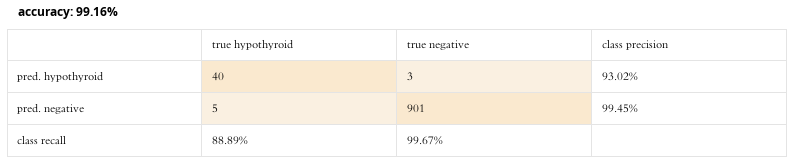
\includegraphics[width=0.75\textwidth]{models/w_j48_performance}
    \caption{Performance del modelo de Árbol generado utilizando el algoritmo C4.5 sobre un conjunto de testeo correspondiente al 30\% del conjunto total de datos.}
    \label{figure:w_j48_performance}
\end{figure}

\begin{figure}[h]
    \centering
    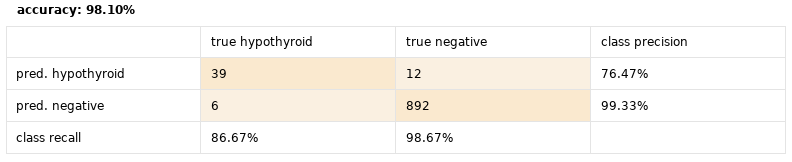
\includegraphics[width=0.75\textwidth]{models/w_oneR_performance}
    \caption{Performance del modelo de reglas generado utilizando el algoritmo OneR sobre un conjunto de testeo correspondiente al 30\% del conjunto total de datos.}
    \label{figure:w_oneR_performance}
\end{figure}

\begin{figure}[h]
    \centering
    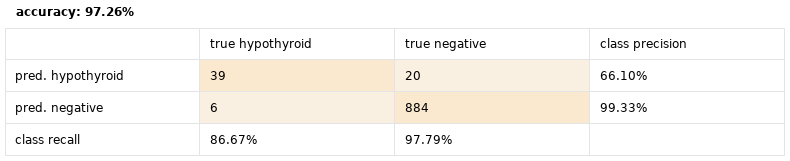
\includegraphics[width=0.75\textwidth]{models/prism_performance}
    \caption{Performance del modelo de reglas generado utilizando el algoritmo PRISM sobre un conjunto de testeo correspondiente al 30\% del conjunto total de datos.}
    \label{figure:prism_performance}
\end{figure}

\begin{figure}[h]
    \centering
    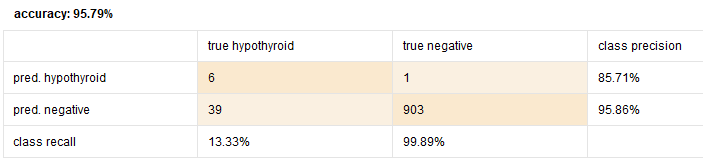
\includegraphics[width=0.75\textwidth]{models/perceptron_performance}
    \caption{Performance del modelo de redes neuronales generado utilizando la arquitectura perceptron sobre un conjunto de testeo correspondiente al 30\% del conjunto total de datos.}
    \label{figure:perceptron_performance}
\end{figure}

\begin{figure}[h]
    \centering
    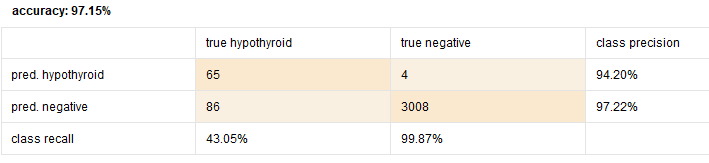
\includegraphics[width=0.75\textwidth]{models/perceptron_train_test_performance}
    \caption{Performance del modelo de redes neuronales generado utilizando la arquitectura perceptron sobre un conjunto de testeo correspondiente conjunto total de datos de entrenamiento.}
    \label{figure:perceptron_train_test_performance}
\end{figure}

\begin{figure}[h]
    \centering
    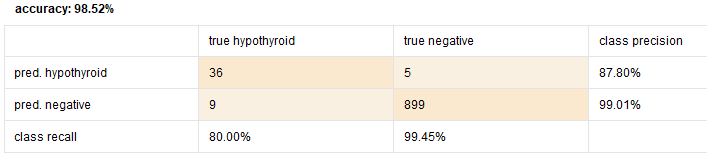
\includegraphics[width=0.75\textwidth]{models/multiperceptron_performance}
    \caption{Performance del modelo de redes neuronales generado utilizando la arquitectura multiperceptron sobre un conjunto de testeo correspondiente al 30\% del conjunto total de datos.}
    \label{figure:multiperceptron_performance}
\end{figure}

\begin{figure}[h]
    \centering
    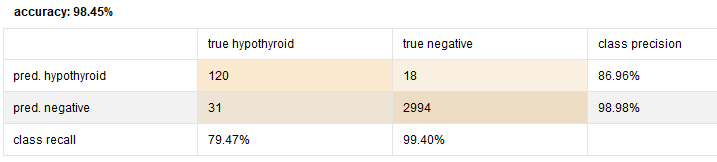
\includegraphics[width=0.75\textwidth]{models/multiperceptron_train_test_performance}
    \caption{Performance del modelo de redes neuronales generado utilizando la arquitectura multiperceptron sobre un conjunto de testeo correspondiente al conjunto total de datos de entrenamiento.}
    \label{figure:multiperceptron_train_test_performance}
\end{figure}

\end{document}
